\appendix
\chapter{Appendices}\label{chap:appendices}
% \section{Non-dimensionalisation}
% The non-dimensionalised incompressible Navier-Stokes equations with Boussinesq approximations for buoyancy describe the motion of a fluid of RBP. 
% % \begin{subequations}\label{eq:rbpdimensional}
% % \begin{equation}
% %     \frac{\partial \mathbf{u^*}}{\partial t^*} + (\mathbf{u^*} \cdot \nabla^*)\mathbf{u^*} = -\frac{1}{\rho}\nabla^* p^* + \nu \nabla^*^2 \mathbf{u^*} + g\gamma(T-T_0)+ \mathbf{f}_b,
% % \end{equation}
% % \begin{equation}
% %     \frac{\partial T}{\partial t^*} + (\mathbf{u^*} \cdot \nabla^*)T= \kappa \nabla^*^2 T,
% % \end{equation}
% % \begin{equation}
% %     \nabla^* \cdot \mathbf{u^*} = 0,
% % \end{equation}
% % with Dirichlet and Neumann boundary conditions.
% % \begin{equation}
% %     \mathbf{u^*}_d, p^*_d, T_d \in \Omega_d, \quad \nabla^*\mathbf{u^*}_N, \nabla^*p^*_N, \nabla^*T_N \in \partial\Omega_N.
% % \end{equation}
% where $\nabla^*=(\partial/\partial x^*, \partial/\partial y^*, \partial/\partial z^*)$ and $t^*$ refer to the differential operators and time with dimensions in per unit space, $m^{-1}$, and time, $s$. $\mathbf{u^*}(\mathbf{x^*}), T(\mathbf{x^*}), p^*(\mathbf{x}^*)$ refers to the three-dimensional fluid velocity, temperature, pressure fields, in dimensional form, while $T_0, \mathbf{f_b}$ refers to a reference temperature and body-forcing terms.
% % For a given set of fluid properties $\rho, \nu, \kappa$ and geometric properties $L^*, t^*, u^*$ referring to an arbitrary length-, time- and velocity-scale, we are primarily interested in the behaviour of the fluid i.e if its laminar or turbulent.
% To reduce the number of control parameters, we can suitably nondimensionalise the primitive variables by a velocity scale $u_c$, length scale, $L_x$, and time scale $u_c/L_x$, where $u_c$ refers to the centreline velocity of a laminar flow and $L_x$ refers to the streamwise length of the domain.
% 
% $\rho, \nu, \kappa, g, \gamma$ refers the fluid's density, kinematic viscosity and thermal diffusivity, gravity, thermal expansion coefficient, properties specific to a given a fluid.
% We note that that for a given pressure gradient, $\Delta P^*$, a laminar centerline velocity forms as $w^*(y^*) = W_{lam}^*(1 - y^2/h^2)$.
% Here, we have a total of nine dimensional quantities $W^*_{lam}, \Delta T, h, \kappa, \nu, \rho, \gamma, g$ that describes the behaviour of the fluid motion.
% However, ultilise the buckingham pi theorem where we can reduce the equations to less dependenc
% \section{Governing equations for Rayleigh-B\'{e}nard convection}\label{app:eqrbc}
% The governing equations for Rayleigh-B\'{e}nard convection are the non-dimensionalised equations with the Boussinesq approximation for buoyancy-driven flow, given by
% \begin{subequations}\label{eq:rbc}
% \begin{equation}
%     \frac{\partial \mathbf{u}}{\partial t} + (\mathbf{u} \cdot \nabla) \mathbf{u} = -\nabla p + Pr\nabla^2 \mathbf{u} + \frac{RaPr}{8}\theta \mathbf{{j}},
% \end{equation}
% \begin{equation}
%     \frac{\partial \theta}{\partial t} + (\mathbf{u} \cdot \nabla) \theta = \nabla^2 \theta,
% \end{equation}
% \begin{equation}
%     \nabla \cdot \mathbf{u} = 0,
% \end{equation}
% \end{subequations}
% subjected to the following boundary conditions at the walls,
% \begin{subequations}\label{eq:bc}
% \begin{equation}
%     \mathbf{u}|_{y=\pm h} = 0, \quad \theta|_{y=-h} = 1, \quad \theta|_{y=h} = 0, 
% \end{equation}
% \end{subequations}
% and the periodic boundary conditions imposed in the planar $x$ and $z$ directions.
% Here, $t$ denotes the time scaled by the vertical thermal diffusion time, $d^2/\kappa$, and $\mathbf{x}(=(x,y,z))$ represents the spatial coordinates non-dimensionalised by depth, $d$.
% The horizontal directions are $x$ and $z$, while $y$ is the vertical direction. 
% The velocity vector is given by $\mathbf{u}(=(u,v,w))$ and is scaled by thermal velocity, $\kappa/d$, $p$.
% The pressure is scaled by $ \rho \kappa^2 / d^2 $, while $\theta(\equiv(T-T_U)/\Delta T)$ refers to the non-dimensional temperature with $T$ being the absolute temperature, and $\mathbf{j}$ denotes the unit vector in $y$-direction. 
% The Rayleigh number $Ra$, and the Prandtl number, $Pr$, are defined as in \S\ref{sec:1}.
% In this study, we set $Pr = 1$.
% 
% \section{Projection methods for Navier-Stokes equations}
% In this section, we describe the projection methods for solving the incompressible Navier Stokes equations.
% The projection methods belong to a general class of splitting methods, where the solution step for obtaining the velocity and pressure from the incompressible Navier Stokes are uncoupled.
% The premise for being able to do this is because the pressure terms act as a Lagrange multiplier which enforces the incompressibility constraint.
% Suppose we want to find the function $u$ that minimises the functional,
% \begin{equation}
% \min_{\mathbf{u} \neq \mathbf{0}} \frac{\nu}{2} (\nabla \mathbf{u}, \nabla \mathbf{u}) - (f, \mathbf{u}), \quad \text{s.t} \quad \nabla \cdot \mathbf{u} = 0
% \end{equation}
% where $(\mathbf{x}, \mathbf{y}) = \int_\Omega \mathbf{x}^T \mathbf{y} \, \mathrm{d}\Omega$ refers to a suitable inner product.
% To solve this optimisation problem, we use the method of Lagrange multipliers which handles the constrain, by converting the equation above into an unconstrained optimisation problem defined by the Lagrangian
% \begin{equation}
% \mathcal{L} = \frac{\nu}{2} (\nabla \mathbf{u}, \nabla, \mathbf{u}) - (f, \mathbf{u}) - (p, \nabla \cdot \mathbf{u})
% \end{equation}
% Taking the variation $\delta \mathcal{L}$, with respect $\delta \mathbf{u}$, we get
% \begin{align}
%     \frac{\delta \mathcal{L}}{\delta \mathbf{u}} &= \nu (\nabla \mathbf{u}, \nabla \delta \mathbf{u}) - (f, \delta \mathbf{u}) - (p, \nabla \cdot \delta\mathbf{u}), \\
%                                                  &= - \nu (\nabla^2 \mathbf{u}, \delta \mathbf{u}) - (f, \delta \mathbf{u}) + (\nabla p, \delta \mathbf{u}) \\
%                                                  & = (-\nu \nabla^2 \mathbf{u} - f + \nabla p , \delta \mathbf{u}).
% \end{align}
% and with respect to $\delta p$, we get,
% \begin{equation}
%     -\frac{\delta \mathcal{L}}{\delta p} = (\delta p, \nabla \cdot \mathbf{u}).
% \end{equation}
% The optimal condition is defined by vanishing variations, hence, we recover the Stokes equations,
% \begin{subequations}
%     \begin{equation}
%         \nu \nabla^2 \mathbf{u} + \nabla p = -f
%     \end{equation}
%     \begin{equation}
%         \nabla \cdot \mathbf{u} = 0        
%     \end{equation}
% \end{subequations}
% In other words, the role of pressure is to serve as a constrain to enforce incompressibility, where we can consider a velocity field that is not divergence fre, which is then corrected by pressure later - the splitting method.
% To witness this is action, we consider the basic approach of Chorin's projection which is a two step method,
% \begin{subequations}
% \begin{equation}
%     \frac{\mathbf{u}^* - \mathbf{u}^n}{\Delta t} = - (\mathbf{u}^n \cdot \nabla) \mathbf{u}^n + \nu \nabla^2 \mathbf{u}^n
% \end{equation}
% \text{then,}
% \begin{equation}
%     \mathbf{u}^{n+1} =  \mathbf{u}^* + {\Delta t} \nabla p^{n+1}.
% \end{equation}
% \end{subequations}
% The idea of projection stems of taking the weak formulation of the second equation with $v \in \mathbf{V} := { \mathbf{v} \in H_0^1(\Omega) \, : \, \nabla \cdot \mathbf{v} = 0 }$,
% \begin{equation}
%     (\mathbf{u}^*, \mathbf{v}) = (\mathbf{u}^{n+1}, \mathbf{v}) + (\nabla p^{n+1}, \mathbf{v})
% \end{equation}
% Taking integration by parts we get,
% \begin{equation}
%     (\mathbf{u}^*, \mathbf{v}) = (\mathbf{u}^{n+1}, \mathbf{v}) - \underbrace{ (p^{n+1}, \nabla \cdot \mathbf{v})}_ {=0},
% \end{equation}
% Hence,
% \begin{equation}
%     (\mathbf{u}^*, \mathbf{v}) = (\mathbf{u}^{n+1}, \mathbf{v})
% \end{equation}

\section{Simulation parameters for $Ra$-$Re$ sweep}\label{app:params}
\begin{table}\scriptsize
\centering
\begin{tabular}{l l l l l l l l}
    Ra & Re & $N_z$ & $dt$ & $T$ & $\frac{d}{\kappa}$\\
    \hline
    \hline
    0	&	1050	&	64	&	0.1	&	8000	&	-    \\
    0	&	2000	&	128	&	0.02	&	3000	&	- \\
    \hline
    2000	&	0	&	64	&	0.05	&	50	&	25       \\
    2000	&	0.1	&	64	&	0.005	&	5	&	25       \\
    2000	&	1	&   64	&	0.01	&	50	&	25       \\
    2000	&	10	&	64	&	0.05	&	50	&	2.5      \\
    2000	&	100	&	64	&	0.1	&	50	&	0.25         \\
    2000	&	500	&	64	&	0.1	&	50	&	0.05         \\
    2000	&	750	&	64	&	0.1	&	50	&	0.033        \\
    2000	&	1000&	64	&	0.1	&	50	&	0.025    \\
    2000	&	1050&	64	&	0.1	&	8000	&	3.81    \\
    2000	&	2000&	128	&	0.02	&	2800	&	0.75 \\
    \hline
    3000	&	0	&	64	&	0.05	&	3000	&	1500     \\
    3000	&	0.1	&	64	&	0.005	&	300	&	1500         \\
    3000	&	1	&	64	&	0.05	&	100	&	50           \\
    3000	&	10	&	64	&	0.05	&	50	&	2.5          \\
    3000	&	100	&	64	&	0.1	&	10000	&	50           \\
    3000	&	500	&	64	&	0.1	&	50	&	0.05             \\
    3000	&	750	&	64	&	0.1	&	50	&	0.033            \\
    3000	&	1000&	64	&	0.1	&	50	&	0.025        \\
    3000	&	1050&	64	&	0.1	&	8000	&	3.81         \\
    3000	&	2000&	128	&	0.02	&	2800	&	0.75 \\
    \hline
    5000	&	0	&	64	&	0.005	&	1200	&	600      \\
    5000	&	0.1	&	64	&	0.001	&	800	&	4000         \\
    5000	&	1	&	64	&	0.01	&	2500	&	1250     \\
    5000	&	10	&	64	&	0.05	&	500	&	25           \\
    5000	&	100	&	64	&	0.1	&	1000	&	5            \\
    5000	&	500	&	64	&	0.05	&	8000	&	8       \\
    5000	&	750	&	64	&	0.05	&	8000	&	5.33     \\
    5000	&	1000&	64	&	0.02	&	8000	&	4    \\
    5000	&	1050&	64	&	0.02	&	8000	&	3.81     \\
    5000	&	2000&	128	&	0.02	&	2800	&	0.75 \\ 
    \hline
    8000	&	0	&	64	&	0.0025	&	600	&	300          \\
    8000	&	0.1	&	64	&	0.0005	&	600	&	3000         \\
    8000	&	1	&	64	&	0.005	&	600	&	300          \\
    8000	&	10	&	64	&	0.05	&	500	&	25           \\
    8000	&	100	&	64	&	0.1	&	5000	&	25           \\
    8000	&	500	&	64	&	0.05	&	10000	&	10       \\
    8000	&	750	&	64	&	0.05	&	8000	&	5.33     \\
    8000	&	1000&	64	&	0.02	&	8000	&	4    \\
    8000	&	1050&	64	&	0.02	&	8000	& 3.81   \\
    8000	&	2000&	128	&	0.02	&	2800	&	0.75 \\
    \hline
    10000	&	0	&	64	&	0.0025	&	1000	&	500      \\
    10000	&	0.1	&	64	&	0.00025	&	800	&	4000         \\
    10000	&	1	&	64	&	0.0025	&	600	&	300          \\
    10000	&	10	&	64	&	0.05	&	12000	&	600      \\
    10000	&	100	&	64	&	0.1	&	8000	&	40           \\
    10000	&	500	&	64	&	0.05	&	8000	&	8        \\
    10000	&	750	&	64	&	0.05	&	8000	&	5.33     \\
    10000	&	1000	&	64	&	0.02	&	8000	&	4    \\
    10000	&	1050	&	64	&	0.02	&	8000	& 3.81   \\
    10000	&	2000	&	128	&	0.02	&	2800	&	0.75 \\
\end{tabular}
\caption{The summary of the spatial and temporal resolution for a given $Re$, $Ra$. $N_z$ denotes the number of Fourier expansions in the $z$-direction. $dt, T, d/\kappa$ denotes the timestep, final time and the final time scaled by the thermal timescale.}
\label{tab:simulations}
\end{table}
The spectral/\emph{hp} quadrilateral element width, heights and polynomial order are kept constant for all simulations, $(\Delta x, \Delta y|_{y=\pm h}, \Delta y|_{y=0}, P) = (0.1\pi,0.0549,0.367,4)$.
To resolve the high gradients, the quadrilateral element heights are bunched near the wall, $\Delta y|_{y=\pm h}$, and expanded in the channel center, $\Delta y|_{y=0}$.
The basis type employed here consists of the modified Jacobi polynomials, known as the \emph{modified} basis (see \S \ref{sec:nm_modalexpansions}).
Table \ref{tab:simulations} describes the number of Fourier expansions, $N_z$, and temporal resolution of 52 numerical experiments at $Re = 0, 0.1, 1, 10, 100, 500, 750, 1000, 1050$, $2000$, and $Ra = 0, 2000, 3000, 5000, 8000, 10000$ with $Pr = 1$ and a large aspect ratio, $\Gamma = 4\pi$. 
The initial conditions of all numerical experiments were sampled from a statistically stationary solution based on the time history of the Nusselt number and shear.
The laminar solution obtained for  $Ra = 0$ , $Re \leq 1000$ has been omitted in table \ref{tab:simulations}.

\section[1st and 2nd order statistics]{First- and second-order statistics of the buoyancy- and shear-driven regime}\label{app:statistics}
\subsection{Buoyancy-driven regime}\label{sec:buoyancydriven}
\begin{figure}
    \centering
    \includegraphics[width=\linewidth]{TransitionalRBP/Figures/PhaseSpace/BuoyancyStatistics.pdf}
    \caption{The wall-normal distribution of temporal and plane- averaged (a) streamwise velocity, (b) temperature, (c) fluctuating wall-normal velocity squared normalised by thermal velocity scale, (d) fluctuating temperature squared and (e) fluctuating span- and streamwise velocities squared normalised by thermal velocity scale of buoyancy-driven regime shaded in red in figure \ref{fig:rarephase}.}
    \label{fig:BuoyancyStatistics}
\end{figure}

We present the first- and second-order statistics of the buoyancy-dominated regime (shaded in red), consisting of the (1) SDC \& ISRs, and (2) ISRs states in figure \ref{fig:BuoyancyStatistics}, illustrating its temporal and plane-averaged streamwise velocity, $\langle w \rangle_{x,z,t}$, temperature, $\langle \theta \rangle_{x,z,t}$, fluctuating wall-normal velocity squared normalised by thermal velocity scale, $\langle \tilde{v} \tilde{v} \rangle_{x,z,t}/u_\kappa^2$, fluctuating temperature squared, $\langle \tilde{\theta}\tilde{\theta} \rangle_{x,z,t}$ and fluctuating span- and streamwise velocities squared normalised by thermal velocity scale, $\langle \tilde{u}\tilde{u} + \tilde{w}\tilde{w} \rangle_{x,z,t}/u_\kappa^2$.
We note that the fluctuating components are defined about a temporal-planar averaged quantity, i.e $\tilde{\mathbf{u}} = \mathbf{u} - \langle \mathbf{u} \rangle_{x,z,t}$.
The mean temperature profiles (figure \ref{fig:BuoyancyStatistics}(b)), and the fluctuating span- and streamwise velocities (figure \ref{fig:BuoyancyStatistics}(f)) are visually similar for the same $Ra$, and are nearly independent of $Re$.
However, we observe the dependence on $Re$ at $Ra = 3000$ in the fluctuating temperature squared (figure \ref{fig:BuoyancyStatistics}(d)), and fluctuating wall-normal velocities (figure \ref{fig:BuoyancyStatistics}(c)), likely due to variations in convection structures, particularly in the convection roll wavenumbers. 
A detailed analysis of how the statistical properties vary with roll wavenumber is beyond the scope of this work.
We propose that the underlying flow structure, consisting of convection rolls, describes the buoyancy-driven regime, shaded in red in figure \ref{fig:rarephase}.
In this regime, the strength of the convection is primarily controlled by $Ra$, akin to RBC, and remains independent of $Re$.

% The influence of $Ra$ and $Re$ on the mean streamwise velocity profile appears to be modest in figure \ref{fig:BuoyancyStatistics}(a).
% Notably, an increase in $Ra$ leads to a slight increase in shear, deviating from the laminar value of 2, illustrated in figure \ref{fig:raredwdynu}. 
\subsection{Shear-driven regime}\label{sec:sheardriven}
\begin{figure}
    \centering
    \includegraphics[width=\linewidth]{TransitionalRBP/Figures/PhaseSpace/ShearStatistics.pdf}
    \caption{The wall-normal distribution of temporal and plane- averaged (a) streamwise velocity, (b) temperature, (c) fluctuating streamwise velocity squared, (d) fluctuating wall-normal velocity squared, (e) fluctuating spanwise velocities squared,  (f) fluctuating Reynolds stresses and (g) fluctuating temperature squared in the shear-driven regime shaded in blue in figure \ref{fig:rarephase}.}
    \label{fig:sheardrivenstatistics}
\end{figure}

As $Re$ falls within the range of $1050 \leq Re \leq 2000$, shear-driven turbulence dominates, where the impact of $Ra$ on the first- and second-order statistics is weakly dependent on $Ra$ in figure \ref{fig:sheardrivenstatistics}.
Figure \ref{fig:sheardrivenstatistics} describes the temporal and plane-averaged streamwise velocity, $\langle w \rangle_{x,z,t}$, temperature, $\langle \theta \rangle_{x,z,t}$, fluctuating streamwise velocity squared, $\langle \tilde{w}\tilde{w} \rangle_{x,z,t}$, fluctuating wall-normal velocity squared, $\langle \tilde{v} \tilde{v} \rangle_{x,z,t}$, fluctuating spanwise velocities squared, $\langle \tilde{u}\tilde{u} \rangle_{x,z,t}$, fluctuating Reynolds stresses $\langle \tilde{v}\tilde{w} \rangle_{x,z,t}$, and fluctuating temperature squared, $\langle \tilde{\theta}\tilde{\theta} \rangle_{x,z,t}$ at $Re = 2000, 1050$ for $Ra \in [0, 10000]$.
The flow structures appear as uniform, featureless turbulence \citep{tuckerman_turbulent-laminar_2014} at $Re = 2000$, independent of $Ra$.
\begin{figure}
    \centering
    \includegraphics[width=\linewidth]{TransitionalRBP/Figures/Appendix/Re2000-BotSpaceTimeCompiled.pdf}
    \caption{Spacetime plots of near-wall, wall-normal and spanwise perturbation kinetic energy for $Re = 2000$, $t\in[0, 2800]$, $\Gamma= 4\pi$ at (a) $Ra = 10000$, (b) $Ra = 8000$, (c) $Ra = 5000$, (d) $Ra = 3000$, (e) $Ra = 2000$, (f) $Ra = 0$.}
    \label{fig:spacetime-Re2000}
\end{figure}
The spacetime figure of near-wall ($y^+ = 15$), wall-normal and spanwise perturbation kinetic energy, $\mathcal{E}_{u'+v'}$, at $Re = 2000$, $t \in [0,2800]$, illustrating spatially uniform featureless turbulence, visually distinguishable withn $Ra \in [0, 10000]$, corroborating with their $Ra$-independent first- and second-order statistics in figure \ref{fig:sheardrivenstatistics}.
In other words, the dominant physical mechanism is shear-driven turbulence at $Re = 2000$, independent of $Ra$.

As $Re$ approaches $Re = 1050$, the midplane temperature in figure \ref{fig:rarephase} shows regions of spatially localised structures, indicating the presence of turbulent-laminar bands, described in figure \ref{fig:spacetime-Ra0k-Re1.05k} and \ref{fig:spacetime-Ra10k-Re1.05k} later.
The mean streamwise velocity and temperature gradients at both ends of the wall, and second-order statistics, are enhanced slightly from $Ra = 0$ to $Ra = 10000$.
This enhancement could be due to the coexistence of longitudinal rolls with turbulent bands at $Ra = 10000$, discussed in \S \ref{sec:rbp_3.3}.
Notably, we have also included the statistics for a subcritical case ($Ra < Ra_{\parallel}$) at $Ra = 1000$, indicating the presence of subcritical effects as the statistics are slightly enhanced from $Ra = 0$ to $Ra = 1000$, reported by \cite{john_soundar_jerome_transient_2012}.
Nonetheless, there is a distinct change of state between $Re = 1000$ to $1050$ (see figure \ref{fig:rarephase}), marked by the transition from the longitudinal/intermittent roll regime to shear-driven turbulence at $Re \geq 1050$, thus, shaded in blue in figure \ref{fig:rarephase}.

% 

% \section{Negligible impact of $Ra$ at $Re = 1800$}\label{app:Re1800}
% \begin{figure}
%     \centering
%     \includegraphics[width=\linewidth]{Figures/RaEffectOnTurbulence/Ra2000-Re1800-BotSpaceTime.pdf}
%     \caption{Spacetime plots of (a) perturbation kinetic energy near the wall, $y^+ = 14.9$ and (b) temperature along $z = 8\pi$ at $Ra = 0, Re=1800$. Midplane snapshots of perturbation kinetic energy, $\frac{1}{2}||\mathbf{u}'||_{y=0}$, and temperature, $\theta|_{y=0}$, at (c,d) $tW_c/h = 2000$, (e,f) $tW_c/h = 4000$ and (g,h) $tW_c/h = 6000$ respectively.}
%     \label{fig:spacetime-Ra2k-Re1.8k}
% \end{figure}
% We present the spacetime plots of the perturbation kinetic energy near the wall, $\frac{1}{2}||\mathbf{u}||^2(x,t)|_{z = \pi, y^+\sim 15}$, midline temperature, $\theta(x,t)|_{z=\pi, y=0}$, and temporal midplane snapshots, $\frac{1}{2}||\mathbf{u}||^2(x,z)|_{t,y^+\sim 15}$, $\theta(x,z)|_{t,y=0}$ at $tU_c/h = 2000, 4000, 6000$ for $Ra = 10000, 0$, $Re = 1800$, for $tW_c/h \in [0, 8000]$, in figures \ref{fig:spacetime-Ra10k-Re1.8k} and \ref{fig:spacetime-Ra2k-Re1.8k} respectively.
% We note that the initial condition of these simulations has been sampled from a statistically stationary turbulent state at $Re = 2000$, which has been slowly reduced to $Re = 1800$, or the desired $Re$ for future simulations.
% The choice of observables is to identify near-wall and midplane flow structures independently, such as near-wall streaks and convection rolls, respectively. %CAUTION: Midplane shows quasistream wise rollers too..
% The choice of observables is to identify the turbulent streaks, typically visible near the wall, separately from the convection rolls, which are visible along the midplane. % Red and blue stripes might not indicate convection rolls..
% At $Re = 1800, Ra = 10000$, the flow structures appear as uniform, featureless turbulence \citep{tuckerman_2020}, in the spacetime perturbation kinetic energy plots, mimicked by the midplane temperature spacetime plots.
% This is further supported by the temporal snapshots of figures \ref{fig:spacetime-Ra10k-Re1.8k}(c-h), revealing a highly disordered turbulent flow field, consisting of possibly many near-wall streaky structures.
% By comparing the results obtained between $Ra = 10000, 2000$ in figures \ref{fig:spacetime-Ra10k-Re1.8k} and \ref{fig:spacetime-Ra2k-Re1.8k}, the flow structures depicting featureless turbulence shown in the spacetime plots (a,b) and temporal snapshots (c-h) are visually similar.
% We suggest that the underlying physical process at $Re = 1800$ is likely shear flow turbulence, regardless of $Ra$.
% This is further supported by the first- and second-order statistics at $Ra = 10000, 2000, 1000, 0$ represented in the figure \ref{fig:Re1800-Ra-Stats} where the impact of $Ra$ is negligible.
% \begin{figure}
%     \centering
%     \includegraphics[width=\linewidth]{Figures/RaEffectOnTurbulence/Re1800-Ra-Statistics.pdf}
%     \caption{A comparison of first- and second-order statistics between $Ra = 10000,2000,1000,0$ at $Re = 1800$. The centreline-velocity normalised wall-normal distribution of (a) streamwise mean velocity, $\langle W \rangle$, (b) mean temperature, $\langle \Theta \rangle$, mean squared (c) streamwise, $\langle \hat{w}\hat{w} \rangle$, (d) wall-normal, $\langle \hat{v}\hat{v} \rangle $, (e) spanwise, $\langle \hat{u}\hat{u} \rangle$, fluctuating velocity, (f) fluctuating Reynolds stresses, $\langle \hat{v}\hat{w} \rangle$ and (g) temperature fluctuations, $\langle \hat{\theta}\hat{\theta} \rangle$ from $y \in [-1, 1]$. The fluctuating components are defined as $\hat{w} = \langle W \rangle - w$, where $\langle \cdot \rangle = \frac{1}{TL_xL_z} \int_{t,x,z} \; \cdot \; \mathrm{d}t\mathrm{d}x\mathrm{d}z$ refers to the temporal and stream- and span-wise spatially averaged operator.}
%     \label{fig:Re1800-Ra-Stats}
% \end{figure}

\section{Growth rates of primary instabilities}\label{app:long-pri}
\begin{figure}
    \centering
    \includegraphics[width=\linewidth]{TransitionalRBP/Figures/Appendix/peigs.pdf}
    \caption{Growth rates of primary instabilities at $Ra = 10000, 8000, 5000, 3000, 2000$ leading to the onset of longitudinal rolls against spanwise wavenumber of $\alpha d$ at $Re = 1050$.}
    \label{fig:long-pri-instab}
\end{figure}

Figure \ref{fig:long-pri-instab} shows the eigenvalues of the primary instabilities as a function of its spanwise wavenumber $\alpha d$, leading to the onset of longitudinal rolls at $Re = 1050$. The results are obtained using a Chebyshev-collocation method discretised by 51 Chebyshev polynomials \citep{driscoll_chebfun_2014}. The crosses denote the spanwise wavenumbers admissible within the domain $\Gamma = \pi/2$, where $\alpha d = 4$ corresponds to the dominant eigenmode.
\section{Verification of linear stability analysis}\label{app:sdc_appA}
\begin{figure}
    \centering
    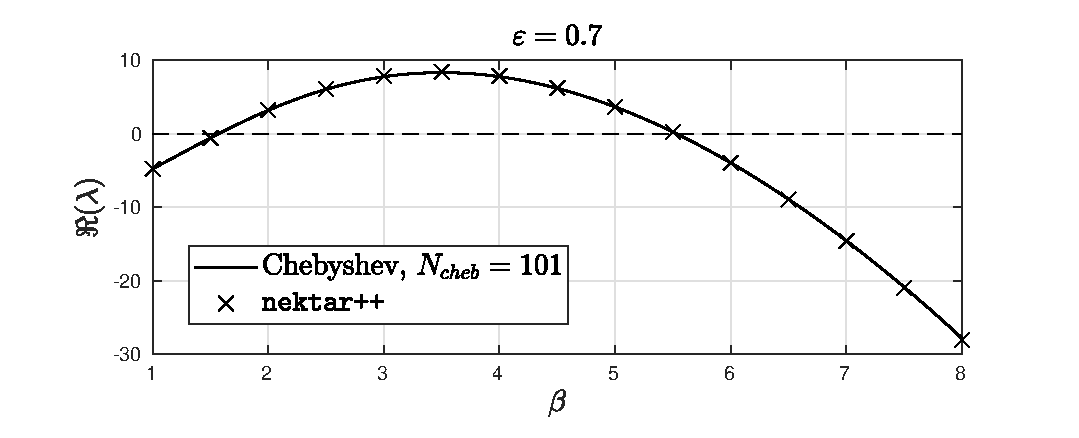
\includegraphics[width=1\textwidth]{StateSpaceStructureOfSDC/Figures/evComparisonPlot.eps}
    \caption{Eigenvalues of primary instabilities of RBC at $\varepsilon = 0.7$ computed in Nektar++ compared against a Chebyshev-collocation method with $101$ Chebyshev expansions.}
    \label{fig:evvalidation}
\end{figure}

Figure \ref{fig:evvalidation} shows the eigenvalues as a function of spanwise wavenumber $\beta$ of RBC at $\varepsilon = 0.7$. The results are obtained using Nektar++ and compared against a Chebyshev-collocation method discretised by 101 Chebyshev polynomials \cite{driscoll_chebfun_2014}.

\section{Other elementary states and ISRs}\label{app:sdc_appB}
Figure \ref{fig:10elementaries} presents snapshots of temperature slices ($\theta(x,z)|_{d/2}$), depicting ten distinct elementary states. These states are obtained within a minimal domain $\Gamma = 2\pi$, consisting of eight stationary states (figures \ref{fig:10elementaries}(a-h)) and two travelling-wave states (figures \ref{fig:10elementaries}(i,j)).
Figure \ref{fig:ISRs} features a snapshot of fourteen ideal straight rolls (ISRs), and they satisfy rotational symmetry about the $y$-axis and mirror symmetries about the $x$- and $z$-axes due to the horizontal isotropy of the present system. These ISRs represent stable fixed-points in the state space of figures \ref{fig:statespace-sdc-isr-transient}, \ref{fig:statespace-sdc-isr-elems}, \ref{fig:statespace-sdc-isr-elems-edge}, \ref{fig:phasespacetraj}.

\begin{figure}
    \centering
    \includegraphics[width=\textwidth]{StateSpaceStructureOfSDC/Figures/elementaries.pdf}
    \caption{Temperature snapshots, $\theta(x,z)|_{y=d/2}$, of 10 elementary states confined within a minimal domain $\Gamma = 2\pi$: (a) steady `forked-A' state, (b) steady `forked-B' state, (c) steady `forked-c' state, (d) steady `twin-armed' state, (e) steady `tri-rolls' state, (f) travelling-wave `O-a' state, (g) travelling-wave `O-b' state, (h) steady `keyhole' state, (i) relative periodic orbit `eye' state, (j) relative periodic orbit `S' state}
    \label{fig:10elementaries}
\end{figure}

\begin{figure}
    \centering
    \includegraphics[width=\textwidth]{StateSpaceStructureOfSDC/Figures/ISRs.pdf}
    \caption{Temperature snapshots, $\theta(x,z)|_{y=d/2}$, of 14 stable ideal straight rolls (ISRs) confined within a minimal domain, $\Gamma = 6.28$. Plots (a-n) are ordered in increasing wavenumbers, $q \in (2/d, 3.35/d)$.}
    \label{fig:ISRs}
\end{figure}
